\section{D7-brane}\label{sec:D7brane}

The holographic dictionary for $N_f$ flavors of quarks in a four-dimensional $SU(N)$ SYM theory is a set of $N_f$ D7-branes in the ten-dimensional supergravity dual. We work in the probe limit, when $N_f/N \rightarrow 0$, meaning the additional branes do not back-react on the background geometry. Furthermore, at this limit, the Landau pole that can potentially develop in the dual theory is strongly suppressed, \cite{CasalderreySolana:2011us}. We study the simplest setting, with $N_f=1$ probe brane \footnote{For many coincident branes in the probe limit, they are non-interacting, hence the non-abelian action that describes them reduces to $N_f$ copies of the abelian action.}.

Our D7-brane embedding wraps the warped $AdS_5$ and the three-dimensional ellipsoid of the deformed $S^5$ of the Pilch-Warner metric. Furthermore, our D7-brane carries no charge, hence no worldvolume gauge field: $F = 0$. This is the equivalent setting studied in \cite{Karch:2002sh} for $AdS_5 \times S^5$, which our configuration will reduce to, near the boundary.


Let us consider the D7-brane worldvolume, induced from the target space with 
\begin{equation}\label{eq:ansatz}
 \theta = \theta(c), \quad \phi=\phi_0\equiv\frac{(2 n + 1)\pi}{2}.
\end{equation}
Our particular choice of $\phi_0$ simplifies our problem, because
\begin{equation}
 P[B_{(2)}] = 0.
\end{equation}
The induced metric from \eqref{eq:PWmetric} with $d\theta = \theta'(c) dc$ and $d\phi=0$ is thus:
\begin{align}\label{eq:D7metric}
ds_{D7}^2 =
v_x^2 dx_\mu dx^\mu 
- (v_c^2 +v_\theta^2 \theta'(c)^2)\, dc^2 - v_1^2 \sigma_1^2 - v_2^2 (\sigma_2^2 + \sigma_3^2),
\end{align}
where we used lower case $v$ to denote the pullback of the target space vielbeins.



%%%%%%%%%%%%%%%%%%%%%%%%%%%%%%%%%%%%%%%%%%%%%%%%%%%%%%%%%%%%%%%%%%%%%%%%%%%%%%%%%%%%%%%%%%%%%%%%%
\subsection{Kappa symmetry projector}

The kappa symmetry projector for our configuration is:
\begin{align}
\Gamma = - \dfrac{ \gamma_{(8)} \mathcal{I} }{\sqrt{-\det g}},
\end{align}
with
\begin{align}
 \gamma_{(8)} = - v_x^4 v_1 v_2^2 \Gamma_{1 2 3 4 7 8 9}( v_c \Gamma_5 +  v_{\theta} \theta'(c) \Gamma_6), 
\end{align}
where we used capital gammas to denote the gamma matrices in the local frame; see appendix \ref{sec:localframe}.

The projector can be further simplified by combining it with the chirality condition, which for the mostly-minus metric convention is: 
\begin{equation}
 \Gamma_{11} \epsilon = -\epsilon, \quad 
 \Gamma_{11} \equiv \Gamma_{12345678910}.
\end{equation}
Then, the supersymmetric condition \eqref{eq:susyCondition} becomes:
\begin{equation}
 \Gamma_{11} \Gamma \epsilon = \epsilon,
\end{equation}
and 
\begin{align} \label{eq:newProjector}
  \mathcal{P}' \equiv \Gamma_{11} \Gamma  = \dfrac{1}{\sqrt{1+\xi^2}}(1- i \xi  \Gamma_{510}), \quad 
   \xi \equiv  \dfrac{v_\theta}{v_c} \theta'(c),
\end{align}
where we have applied $\mathcal{I} \epsilon = -i\epsilon$ and $\Gamma_{610} \epsilon = -i \epsilon$. The latter identity is due to $\mathcal{P}_- \epsilon = 0$, which is straightforward to show, and the projector is defined in \eqref{eq:projectors}.


%%%%%%%%%%%%%%%%%%%%%%%%%%%%%%%%%%%%%%%%%%%%%%%%%%%%%%%%%%%%%%%%%%%%%%%%%%%%%%%%%%%%%%%%%%%%%%%%%
\subsection{Supersymmetric condition}

For the Killing spinor \eqref{eq:KillingSpinor}, the invertible operator in \eqref{eq:susyCondition0} is:
\begin{align}
 \mathcal{O} &= \exp{\left(\frac{\alpha}{2}\Gamma_{56} \right)} \exp{\left(-\frac{\phi}{2}\, \Gamma_{610} \right)} \exp{\left(\frac{\beta}{2}\Gamma_{710} \mathcal{K} \right)} \\
 \mathcal{O}^{-1} &=  \exp{\left(-\frac{\beta}{2}\Gamma_{710} \mathcal{K} \right)} 
 \exp{\left(\frac{\phi}{2}\, \Gamma_{610} \right)} 
 \exp{\left(-\frac{\alpha}{2}\Gamma_{56} \right)}.
\end{align}


The kappa symmetry projector contains the operator $\mathcal{I}$, which can be replaced as follows (see notation in \ref{sec:KillingSpinor}):
\begin{equation}
 \mathcal{I}\eta =-i \eta = \Gamma_{610} \eta,
\end{equation}
where we used $\mathcal{P}_- \eta =0$ in the last step. 

Then, \eqref{eq:susyCondition0} reduces to:
\begin{equation}
 \Pi_{-} \mathcal{O}^{-1} \gamma_{(8)} \mathcal{O} \Gamma_{610} \Pi_{+}  = 0.
\end{equation}
which, after manipulating the gamma matrices, gives:
\begin{equation}
i v_1 v_2^2 v_x^4 \Pi_- \Gamma_{6 8 9 10} \mathcal{K} \sin\beta \left(v_c \sin\alpha - v_\theta \cos\alpha \, \theta'(c)\right) = 0
\end{equation}
Therefore, the condition our configuration must satisfy in order to preserve supersymmetry is:
\begin{equation}\label{eq:susyConditionTheta}
 \theta'(c) = \dfrac{v_c}{v_\theta} \tan\alpha = \dfrac{c \, \tan\theta(c)}{c^2-1} .
\end{equation}


One can repeat the analysis of \eqref{eq:susyCondition0} for the other projector $\mathcal{P}_{\pm}$, and it will give the same condition \eqref{eq:susyConditionTheta}.


The projector \eqref{eq:newProjector} at the solution \eqref{eq:susyConditionTheta} is simply
\begin{equation}
\mathcal{P}' = \cos \alpha - i \sin \alpha \, \Gamma_{510},
\end{equation}
since $ \xi =  \tan \alpha $.
No more projectors are found, therefore, ours is a 1/2-BPS embedding.


\subsection{Solution}\label{sec:solution}

The solution to the differential equation \eqref{eq:susyConditionTheta} is:
\begin{equation}\label{eq:susyConditionSolution}
\boxed{\sin\theta(c) = L \sqrt{c^2-1}; \quad 1 < c \leq \sqrt{1+L^{-2}}},
\end{equation}
where $L$ is an integration constant. As we will show below, it is the asymptotic separation of the D7-brane from the stack of the D3-branes, in the units of the spherical radius\footnote{The spherical part of our metric \eqref{eq:PWmetric} is multiplied by $R^2$.} $R$, namely $L$ above is really $ L/R$.
We have set $R=1$ so far. The upper bound of $c$ is set by the maximum of the sine.


Near the boundary, $c \approx 1 + z^2/2$, the solution behaves as
\begin{equation} \label{eq:thetaExpanded}
 \theta(z) \approx L \, z + \left(\frac{L}{8} +\frac{L^3}{6} \right) \, z^3 + O(z^5).
\end{equation} 
Moreover, keeping only the leading order of the large $L$ expansion, our solution reduces to the one found in the $AdS_5 \times S^5$ background, see \cite{Karch:2002sh} and \cite{Karch:2005ms}, i.e.
\begin{equation}
 \sin\theta(z)_\text{AdS} = L z,
\end{equation}
with the asymptotic expansion
\begin{equation}
\theta(z)_\text{AdS} \approx L z + \frac{L^3}{6} z^3 + O(z^5).
\end{equation}
The $L\gg 1$ limit ensures the upper bound for $c$ in \eqref{eq:susyConditionSolution} to reduce to the one from the AdS solution, namely $z_\text{max}=1/L$. 


As \cite{Karch:2005ms} explains, in the flat embedding space limit, this embedding describes a planar D-brane located at a constant distance $L$ away from the stack of $N$ D3-branes:
\begin{equation}
 L = \lim_{z \rightarrow 0 } \frac{R}{z} \sin\theta(z) = R \, L/R,
\end{equation}
where we explicitly stated $R$. Furthermore, this separation is proportional to the quark mass $m$:
\begin{equation}
 L = 2 \pi l_s^2 m.
\end{equation}


Figures in \ref{fig:vielbeins} show the vielbeins of the induced metric at the solution, from which we learn how the geometry of the embedding looks like at different values of $c$. First, observe the divergence at the horizon $c_\text{max}=\sqrt{1+L^{-2}}$. This is the location of the well-known enhançon locus, at $\theta = \pi/2$, see \cite{Buchel:2000cn} and \cite{Evans:2000ct}. The spheroid is undeformed at the boundary $c=1$, and becomes squashed until it vanishes at the enhançon. 

\begin{figure}[t!]
\begin{center}
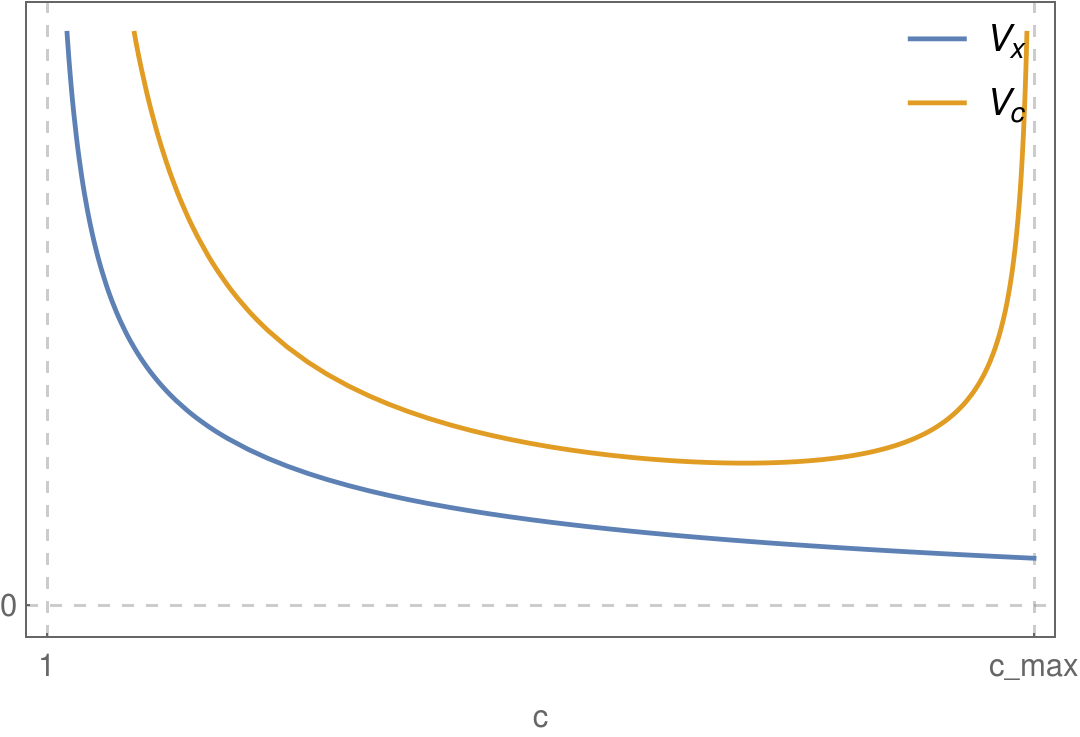
\includegraphics[width=0.6\textwidth]{pictures/vxvcb.png}
\end{center}
\vspace{0.05mm}
\begin{center}
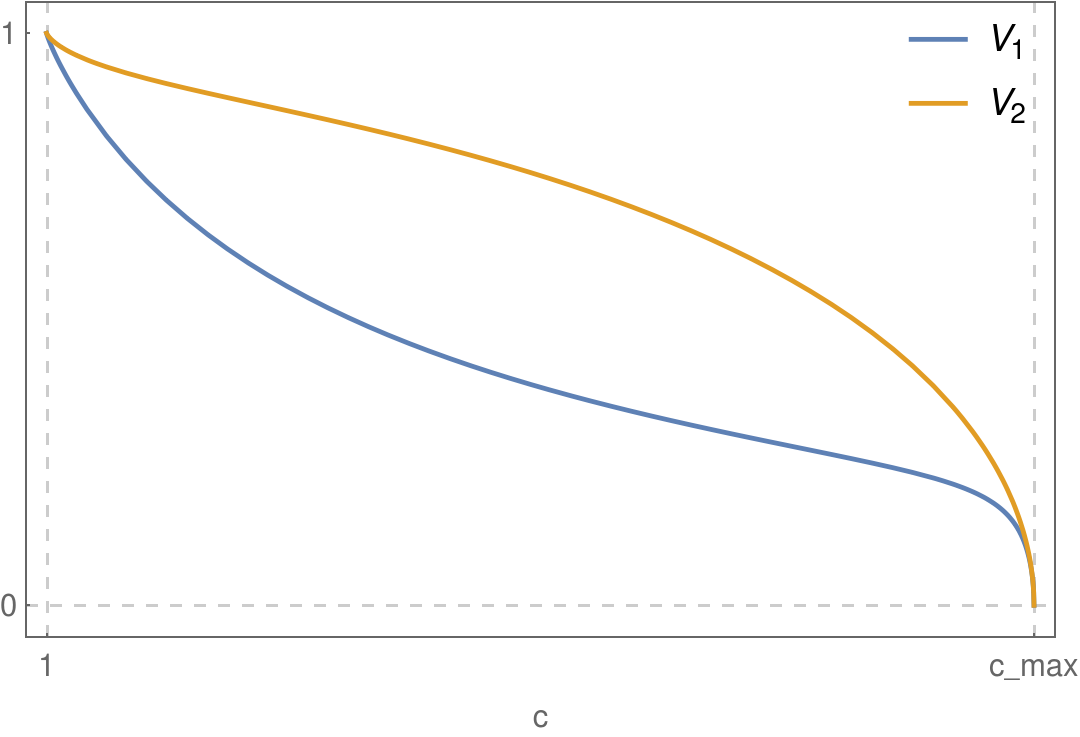
\includegraphics[width=0.6\textwidth]{pictures/v1v2b.png}
\end{center}
\caption{\label{fig:vielbeins} The vielbeins of the induced metric for the allowed values of $c$.}
\end{figure}

